% !TEX root = TD_fluides_part2.tex

\section{Ecoulements en conduite}

\setcounter{subsection}{-1}



\subsection{Transvasement}

{\em Enoncé et correction sur Moodle } 


%--------------------------------------------------------------------------------------------------
\subsection{Ecoulement dans une galerie}
%--------------------------------------------------------------------------------------------------

On consid\`ere l'\'ecoulement dans une galerie horizontale d'am\'enagement hydro\'electrique, de diam\`etre $D = 4$ m et de longueur $L = 16$ km, entre la base d'une retenue d'eau, situ\'ee \`a la profondeur $H = 100$ m sous la surface libre, et un r\'eservoir qu'on consid\`erera, pour simplifier, \`a la pression atmosph\'erique. Il s'agit ici de d\'eterminer quel est le ph\'enom\`ene qui d\'etermine la vitesse moyenne $U$ de l'\'ecoulement dans la galerie~: l'inertie du fluide dans la retenue, ou la dissipation visqueuse dans la galerie (coeffcient de perte de charge $\Lambda$, la dissipation dans la retenue est n\'egligeable).

\begin{enumerate}
\item Montrer que si la longueur de la galerie est sup\'erieure \`a une longueur critique $L_c(D, \Lambda)$, la vitesse est d\'etermin\'ee par la perte de charge. Cette condition est-elle v\'erifi\'ee ici~? 
\item En consid\'erant que le r\'egime d'\'ecoulement est ``hydrauliquement rugueux'' ($Re > 10^5$), condition que l'on v\'erifiera {\it a posteriori}, d\'eterminer la vitesse de l'\'ecoulement dans la galerie. On rappelle que dans le r\'egime rugueux, le coefficient de perte de charge ne d\'epend plus du nombre de Reynolds, et est donn\'e par la formule de Colebrook simplifi\'ee (encore appel\'ee formule de Karman-Prandtl ou de Karman-Nikuradse)~:
$$
\frac{1}{\sqrt{\Lambda}} = 2 \log_{10} \frac{3,71 \, D}{k},
$$
o\`u on prendra $k = 300$ mm pour la rugosit\'e de la galerie. 
\item La vitesse de l'\'ecoulement est-elle peu sensible ou tr\`es sensible \`a la rugosit\'e~? (On pourra \'evaluer la diminution relative de vitesse lorsque la rugosit\'e est multipli\'ee par 5, de 100 \`a 500 mm par exemple.)
\end{enumerate}

%Solution : \\
%galerie : $p_0 - p_a = \Lambda \frac{L}{D} \frac{\rho U^2}{2}$ \\
%retenue : $p_a + \rho g H = p_0 + \frac{\rho U^2}{2}$ \\
%d'o\`u $L_c$. \\
%$\Lambda L/D = 0,087 \times 4000 = 348 \gg 1$, d'o\`u $U = 2,4$ m/s, $Re \approx 10^7$. Pour $k = 100$ et 500 mm, $U = 3,0$ et 2,1 m/s. La vitesse diminue de 30\% quand la rugosit\'e est multipli\'ee par 5~: peu sensible.


%--------------------------------------------------------------------------------------------------
\subsection{Elargissement brusque}
%--------------------------------------------------------------------------------------------------

On s'int\'eresse dans cet exercice à l'\'ecoulement dans une conduite au passage d'un
\'elargissement brusque.
L'\'ecoulement dans la section $S_1$ en amont de l'\'elargissement a une vitesse $u_1$ 
et une pression $p_1$ suppos\'ees connues.
On cherche à d\'eterminer la vitesse $u_2$ et la pression $p_2$
au niveau d'une section $S_2$ en aval de l'\'elargissement (fig.~\ref{fig:elargissement1}a).
On notera $s = S_1/S_2 < 1$, $S_1$ et $S_2$ correspondant aux aires des sections
de part et d'autre de l'\'elargissement, suppos\'ees connues.
On supposera que, bien que turbulent, l'\'ecoulement est stationnaire en moyenne.
Le fluide est homogène, de masse volumique $\rho$ uniforme, et sans perte de
g\'en\'eralit\'e, on n\'egligera la pesanteur.
La paroi de la conduite est imperm\'eable.

\begin{figure}[htb]
  \begin{center}
	\setlength{\unitlength}{0.8mm}
    \begin{picture}(190, 35)(10, 1)
      \put(7, 5){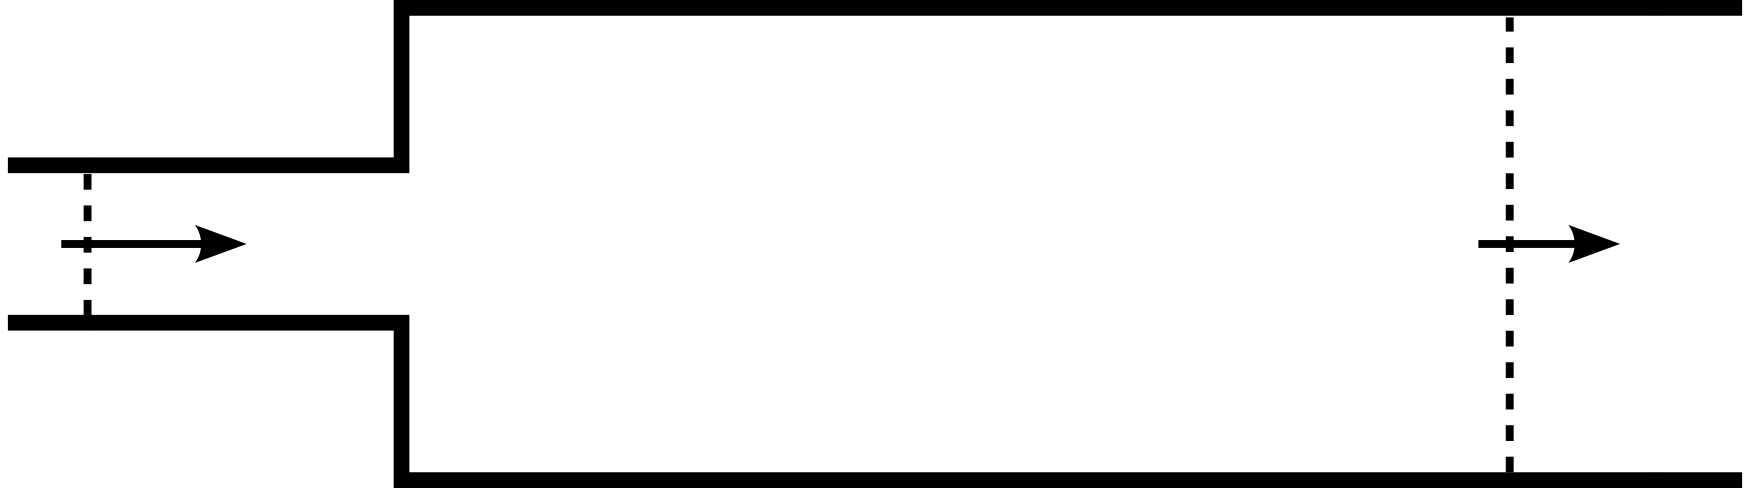
\includegraphics[width=72mm]{elargissement1.png}}
      \put(0, 17){\small $u_1, p_1$}
      \put(92, 17){\small $u_2, p_2$}
      \put(10, 8){\small $S_1$}
      \put(83, 0){\small $S_2$}
      \put(50, 31){\small $\Sigma$}

      \put(117, 5){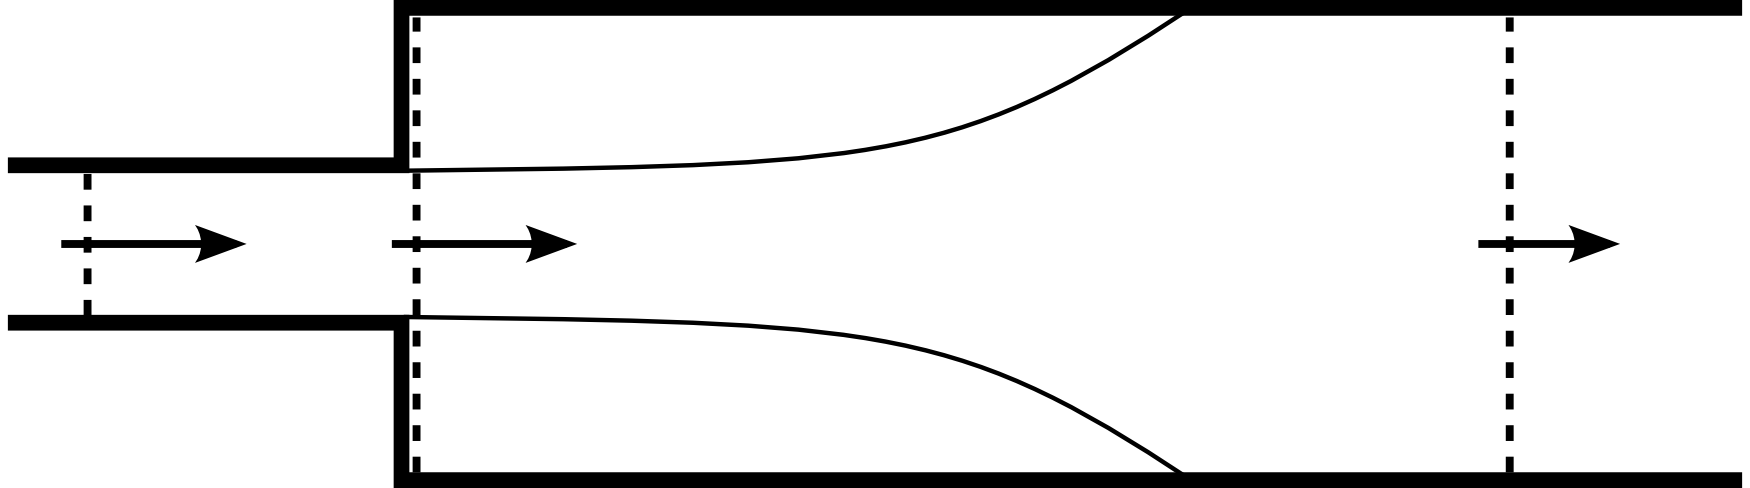
\includegraphics[width=72mm]{elargissement2.png}}
      \put(110, 17){\small $u_1, p_1$}
      \put(148, 17){\small $u_1', p_1'$}
      \put(202, 17){\small $u_2, p_2$}
      \put(120, 8){\small $S_1$}
      \put(137, 0){\small $S_1'$}
      \put(193, 0){\small $S_2$}
      \put(160, 31){\small $\Sigma$}
      \put(141, 25){\small $u \approx 0, p \approx p_1'$}

			\put(50, -4){(a)}
			\put(160, -4){(b)}

   \end{picture}
  \end{center}
  \mycaption{Elargissement brusque dans une conduite : sch\'ema global (a) et d\'etail de l'\'ecoulement d\'ecoll\'e observ\'e exp\'erimentalement (b).}
  \label{fig:elargissement1}
\end{figure}

\begin{enumerate}
\item
  D\'eterminer $u_2$ en fonction de $u_1$ et $s$.
\item
  On n\'eglige dans cette question les effets visqueux et les pertes de charge.
  \begin{enumerate}
  \item
    Quelle quantit\'e physique est conserv\'ee entre les sections $S_1$ et $S_2$ ?
  \item
    En d\'eduire que $p_2 = p_1 + \rho u_1^2 \, f(s)$ o\`u $f(s)$ est à d\'eterminer.
  \item
    En \'ecrivant le bilan int\'egral de quantit\'e de mouvement dans le volume de contrôle
    d\'elimit\'e par la paroi $\Sigma$ de la conduite et les sections $S_1$ et $S_2$,
    montrer que la force exerc\'ee par l'\'ecoulement sur la paroi $\Sigma$ est de la forme
    $F = (S_1 - S_2) \, g(\rho, u_1, p_1, s)$ o\`u $g$ est une fonction à d\'eterminer. 
  \end{enumerate}
\item
  L'exp\'erience montre que la pression $p_2$ pr\'edite pr\'ec\'edemment surestime la r\'ealit\'e
  et que les pertes de charges sont à prendre en compte imp\'erativement après l'\'elargissement.
  En outre, on observe au niveau de l'\'elargissement un d\'ecollement de l'\'ecoulement qui conduit 
  à la formation d'une zone de recirculation dans laquelle la vitesse est n\'egligeable
  (fig.~\ref{fig:elargissement1}b).
  \begin{enumerate}
  \item
    Les pertes de charge restant n\'egligeables entre $S_1$ et la section $S_1'$
    juste après l'\'elargis\-sement, calculer $u_1'$ et $p_1'$.
  \item
    Après l'\'elargissement, on ne peut plus n\'egliger les pertes de charge.
    En consid\'erant le volume de contrôle d\'elimit\'e par les sections dans le fluide $S_1'$
    et $S_2$ et la portion de paroi entre ces deux sections, montrer que 
    $p_2 = p_1 +  \rho u_1^2 \, h(s)$, o\`u $h(s)$ est à d\'eterminer.
  \item
    En d\'eduire que les pertes de charge entre $S_1'$ et $S_2$ s'\'ecrivent
    $\Delta = \rho u_1^2 \,\delta(s)$, o\`u $\delta(s)$ est une fonction à d\'eterminer.
  \item
    Calculer la force exerc\'ee par l'\'ecoulement sur la paroi $\Sigma$ entre $S_1$ et $S_2$.
  \end{enumerate}
\end{enumerate}




%--------------------------------------------------------------------------------------------------
\subsection{Recherche d'un r\'egime d'\'ecoulement \exonormal}
%--------------------------------------------------------------------------------------------------

D\'eterminer le r\'egime d'\'ecoulement (laminaire, turbulent lisse ou turbulent rugueux) 
et le coefficient de perte de charge $\Lambda$ d'un \'ecoulement d'eau 
($\nu = 10^{-6}$ m$^2$/s \`a 15°C) dans les deux cas suivants : 

% \cite[ex. 78]{Com92} :
% \footnote{D'apr\`es Comolet R. 1992 {\it M\'ecanique exp\'erimentale des fluides}, 
% tome 3, exercice 78, Masson.}~:

\begin{enumerate}
\item 
  Tube de verre de diam\`etre $D = 2$ cm et de rugosit\'e $k = 0,2 \mu$m, 
  d\'ebit $Q_v = 0,6$ litre par seconde.
\item 
  Tuyauterie de fonte de diam\`etre $D = 60$ cm et de rugosit\'e $k = 0,3$ mm, 
  d\'ebit $Q_v = 0,85$ m$^3$/s.
\end{enumerate}

On rappelle qu'en \'ecoulement turbulent, le coefficient de perte de charge est donn\'e par 
la formule semi-empirique de Colebrook
$$
  \frac{1}{\sqrt{\Lambda}} = - 2 \log_{10} 
    \left( \frac{k/D}{3,71} + \frac{2,51}{Re \sqrt{\Lambda}} \right).
$$
Une premi\`ere estimation de $\Lambda$ peut \^etre obtenue en ne retenant que le terme dominant 
dans l'argument du logarithme, en consid\'erant que $\Lambda$ est tr\`es g\'en\'eralement compris 
entre 0,01 et 0,04. 
Une deuxi\`eme estimation peut \^etre obtenue en ins\'erant la premi\`ere dans le logarithme, 
et ainsi de suite. 

%--------------------------------------------------------------------------------------------------
\subsection{Ecoulement dans un ol\'eoduc \exonormal}
%--------------------------------------------------------------------------------------------------

On consid\`ere un \'ecoulement d'huile dans un ol\'eoduc horizontal de diam\`etre $D = 10$ cm 
et de longueur $L = 10$ km. 
Le d\'ebit d'huile est $Q_v = 50$ m$^3$/heure, sa densit\'e est $\rho = 950$ kg/m$^3$ 
et de viscosit\'e dynamique $\mu = 0,2$ Pa\,s.

\begin{enumerate}
\item 
  L'\'ecoulement est-il laminaire ou turbulent~? 
  D\'eterminer la perte de charge et le coefficient de perte de charge $\Lambda$.
\item 
  D\'eterminer la puissance dissip\'ee dans la conduite 
  (on pourra utiliser le th\'eor\`eme de l'\'energie cin\'etique).
\item 
  Pour limiter l'\'epaisseur et donc le coût de la conduite, on d\'esire que la pression 
  ne d\'epasse nulle part 5 MPa. Quelle solution peut-on proposer~?
  % \cite[ex. 68]{Com92} 
  % \footnote{D'apr\`es Comolet R. 1992 {\it M\'ecanique exp\'erimentale des fluides}, 
  % tome 3, exercice 68, Masson.}
\end{enumerate}



